

\begin{table}[H]
\begin{flushleft}\emph{\textbf{Use Case}}\end{flushleft}
\footnotesize
\centering
\settowidth\tymin{\textbf{Entry Condition}}
\setlength\extrarowheight{2pt}
\begin{tabulary}{\textwidth}{|J|J|}
\hline
Name            & ReportViolation \\
\hline
Actors          & Registered User \\
\hline
Entry Condition & The user witnessed a traffic violation which he wants to report \\
\hline
Event Flow      & 
\begin{minipage}[t]{0.7\textwidth}
\begin{enumerate} 
\item In the homepage, the user takes a photo of the violating vehicle
\item The user verifies that the image is clear and the license number is visible
\item The user clicks on the “Continue” button to go on with the processes
\item The user is presented with the page for completing the details of the report
\item The detected plate number is shown
\item The user chooses the type of the violation he is reporting from the available choices
\item The detected user location is shown
\item The user verifies that all the data in the report are right
\item The user clicks the “submit” button
\end{enumerate}
\end{minipage}\\
\hline
Exit Condition  & The user report is submitted to the server and stored in user report history \\
\hline
Exceptions      & 
\begin{minipage}[t]{0.8\textwidth}
\begin{itemize} 
\item The user has not logged in before: The user is redirected to the “GivePermission” functionality
\item The user has denied access in their first login:   The user redirected to the “GivePermission” functionality
\item The image is not clear or the license plate number is not visible in it: The user clicks the “take another” button to take another photo
\item The type of violation is not in the available choices: The user chooses the “other” option and specifies the type of violation by typing it in
\item The detected data fields (plate number and location) is not accurate: The user clicks on the “redetect” button associated to that field The erroneous field is redetected\\
\end{itemize}
\end{minipage}\\
\hline
Special Req     & 
\begin{minipage}[t]{0.8\textwidth}
\begin{itemize}
\item \{NFR\textsubscript{1}\} The detection of plate number must be done in less than 1 second
\item \{NFR\textsubscript{2}\} The detected plate number is accurate 99\% of the time
\end{itemize}
\end{minipage}\\
\hline
\end{tabulary}
\caption{\label{tab:report-usecase}Usecase for Report Violation}
\end{table}

The sequence of steps the the user performs in order to complete the violation report process are represented in the following diagram. The user starts by taking images of the report from which the plate number is detected. After which, the type of the violation selected and the location is detected using the user's location. Finally, the report is submitted.

%***place holder for report-violation-sd***

\begin{figure}[H]
\begin{flushleft}\emph{\textbf{Sequence Diagram}}\end{flushleft}
\caption{Sequence Diagram for Report Violation}
\label{fig:report-violation-SD}
\centering
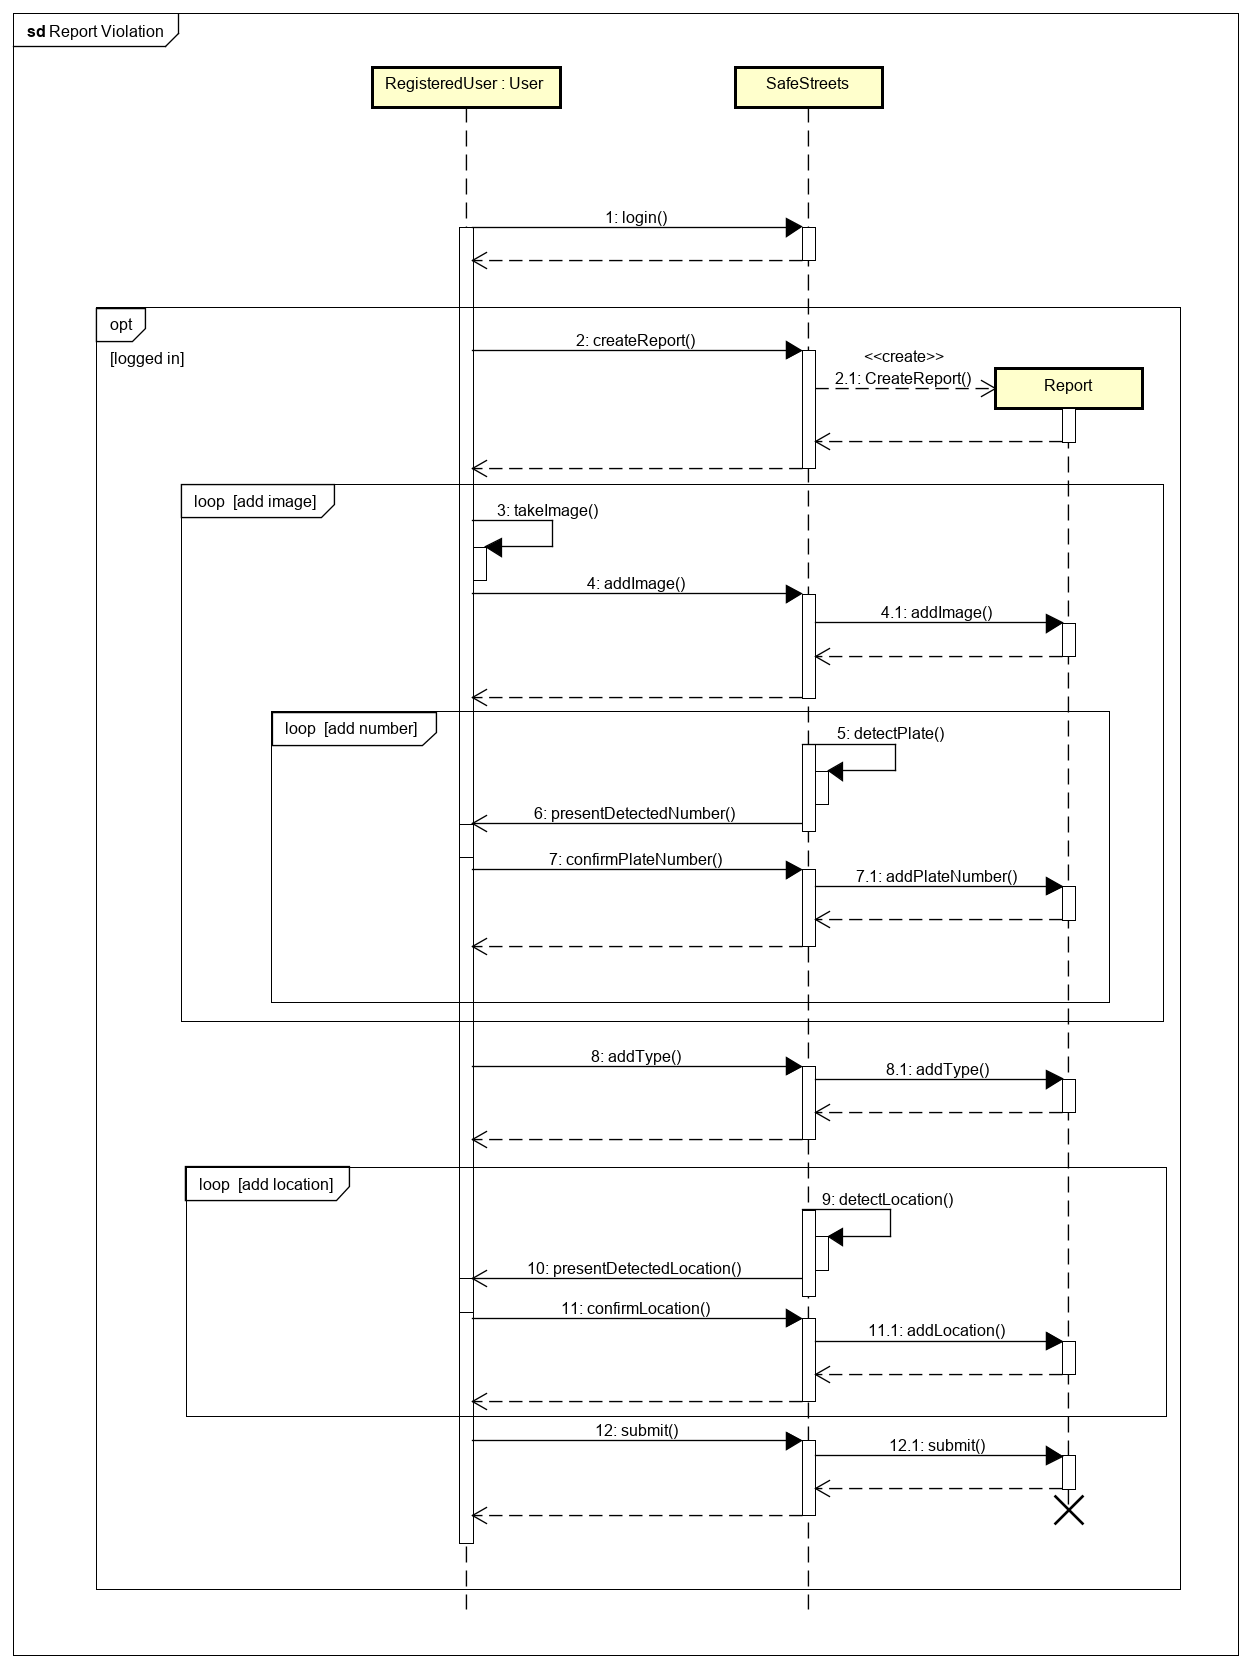
\includegraphics[width=\textwidth, height=0.90\textheight]{report-violation-SD.png}
\end{figure}


